% 广东工业大学本科生毕业设计(论文)LaTeX模板
% 根据《广东工业大学本科生毕业设计(论文)格式规范》制作

\documentclass[12pt,a4paper]{article}
\usepackage[UTF8]{ctex} % 中文支持
% 字体选择：仅在 XeLaTeX 或 LuaLaTeX 下使用 fontspec
\usepackage{ifxetex,ifluatex}
\ifnum\ifxetex1\else0\fi=1
    \usepackage{fontspec}
\else
    \ifnum\ifluatex1\else0\fi=1
        \usepackage{fontspec}
    \else
        \usepackage{times} % 对于 pdfLaTeX 保持传统字体设置
    \fi
\fi
\usepackage{geometry} % 页面设置
\usepackage{circuitikz} % 电路图支持
\usepackage{titlesec} % 标题格式设置
\usepackage{fancyhdr} % 页眉页脚设置
\usepackage{setspace} % 行距设置
\usepackage{graphicx} % 图片支持
\usepackage{amsmath} % 数学公式
\usepackage{amssymb} % 数学符号
\usepackage{booktabs} % 表格美化
\usepackage{array} % 表格支持
\usepackage{multirow} % 表格合并
\usepackage{longtable} % 长表格
\usepackage{cite} % 参考文献引用
\usepackage{enumitem} % 列表环境设置
\usepackage{indentfirst} % 首行缩进
\usepackage{float} % 浮动体控制
\usepackage{caption} % 图表标题
\usepackage{subcaption} % 子图
\usepackage{hyperref} % 超链接
\usepackage{tikz}
\usetikzlibrary{positioning, arrows.meta, calc, backgrounds, fit, shapes.misc, shapes.geometric} % TikZ 库
% 引用显示为方括号内的上标（整体上标），在 hyperref 之后定义为稳健命令
\makeatletter
\DeclareRobustCommand{\brsupcite}[1]{\textsuperscript{[\citen{#1}]}}
\makeatother
\let\oldcite\cite
\renewcommand{\cite}[1]{\brsupcite{#1}}
\usepackage{pdfpages} % 插入PDF封面
\usepackage{listings} % 代码块支持
\usepackage{xcolor} % 代码高亮支持
\usepackage{titlesec}
\titleclass{\subsubsubsection}{straight}[\subsubsection]

% 设置格式
\titleformat{\subsubsubsection}
  {\normalfont\normalsize\bfseries}{\thesubsubsubsection}{1em}{}
\titlespacing*{\subsubsubsection}{0pt}{3.25ex plus 1ex minus .2ex}{1.5ex plus .2ex}

% 设置编号
\newcounter{subsubsubsection}[subsubsection]
\renewcommand\thesubsubsubsection{\thesubsubsection.\arabic{subsubsubsection}}
% 代码块设置
\lstset{
    language=Verilog,
    basicstyle=\ttfamily\scriptsize,
    keywordstyle=\color{blue}\bfseries,
    stringstyle=\color{red},
    commentstyle=\color{green!60!black},
    numbers=left,
    numberstyle=\tiny\color{gray},
    frame=single,
    framesep=5pt,
    breaklines=true,
    breakatwhitespace=false,
    tabsize=2,
    showstringspaces=false,
    captionpos=b,
    abovecaptionskip=10pt,
    belowcaptionskip=10pt
}
\tikzstyle{startstop} = [rectangle, rounded corners, minimum width=3cm, minimum height=1cm,text centered, draw=black]
\tikzstyle{io} = [trapezium, trapezium left angle=70, trapezium right angle=110, minimum width=3cm, minimum height=1cm, text centered, draw=black]
\tikzstyle{process} = [rectangle, minimum width=3cm, minimum height=1cm, text centered, draw=black]
\tikzstyle{decision} = [diamond, minimum width=3cm, minimum height=1cm, text centered, draw=black]
\tikzstyle{arrow} = [thick,->,>=stealth]

% 页面设置
\geometry{
    top=30mm,
    bottom=25mm,
    left=30mm,
    right=20mm
}

% 行距设置：1.5倍行距
\onehalfspacing

% 字体设置（为确保 \textbf 生效，显式设置粗体字体）
% 字体设置（若使用 XeLaTeX/LuaLaTeX 则设定 fontspec 字体）
\ifnum\ifxetex1\else0\fi=1
    \setmainfont{Times New Roman}[BoldFont={Times New Roman}, ItalicFont={Times New Roman Italic}]
    \setCJKmainfont[BoldFont={SimHei}]{SimSun} % 宋体，粗体使用 SimHei
    \setCJKfamilyfont{hei}{SimHei} % 黑体
\else
    % pdfLaTeX: 保持默认字体设置，\textbf 在常规字体下可用
\fi
\newcommand{\hei}{\CJKfamily{hei}}

% 字号定义
\newcommand{\erhao}{\zihao{2}}
\newcommand{\sanhao}{\zihao{3}}
\newcommand{\sihao}{\zihao{4}}
\newcommand{\xiaosi}{\zihao{-4}}
\newcommand{\xiaowu}{\zihao{-5}}

% 表格注释命令
\newcommand{\note}[1]{\par\vspace{0.5em}\noindent\small #1}

% 表格和图像按章节编号设置
\renewcommand{\thetable}{\thesection.\arabic{table}}
\renewcommand{\thefigure}{\thesection.\arabic{figure}}

% 每章开始时重置表格和图像计数器
\makeatletter
\@addtoreset{table}{section}
\@addtoreset{figure}{section}
\makeatother

% 表格标题格式设置：五号黑体加粗，表序与表名之间空一格
\captionsetup[table]{
  font={bf, small},
  labelfont={bf, small},
  labelsep=space,
  justification=centering
}

% 图像标题格式设置：五号宋体，图号与图名之间空一格
\captionsetup[figure]{
  font={small},
  labelfont={bf, small},
  labelsep=space,
  justification=centering
}

% 标题格式设置
\titleformat{\section}{\centering\hei\bfseries\sanhao}{\thesection}{1em}{}
\titleformat{\subsection}{\hei\bfseries\sihao}{\thesubsection}{1em}{}
\titleformat{\subsubsection}{\hei\bfseries\xiaosi}{\thesubsubsection}{1em}{}
\titleformat{\subsubsubsection}{\hei\bfseries\xiaosi}{\thesubsubsubsection}{1em}{}

% 增加标题深度支持
\setcounter{secnumdepth}{4}
\setcounter{tocdepth}{4}

% 段落格式
\setlength{\parindent}{2em} % 首行缩进2字符
\setlength{\parskip}{0pt} % 段间距为0

% 页眉页脚设置
\pagestyle{fancy}
\fancyhf{}
\fancyfoot[R]{\xiaowu\thepage} % 页码位于页脚右侧，小五号
\renewcommand{\headrulewidth}{0pt} % 去掉页眉横线

% 封面设置
% 封面设置（仅当封面文件存在时插入，避免编译因找不到文件失败）
\newcommand{\makecover}{%
      \IfFileExists{论文封面.pdf}{\includepdf[pages=-]{论文封面.pdf}}{}%
}

% 中英文摘要环境
\newenvironment{abstractcn}{
    \begin{center}
        \hei\bfseries\sanhao 摘要
    \end{center}
    \addcontentsline{toc}{section}{摘要}
}{\par}

\newenvironment{abstracten}{
    \begin{center}
        \textbf{\sanhao Abstract}
    \end{center}
    \addcontentsline{toc}{section}{Abstract}
}{\par}

% 关键词命令
\newcommand{\keywords}[1]{
    \vspace{\baselineskip}
    {\hei\bfseries\sihao 关键词：} #1
}

\newcommand{\keywordsen}[1]{
    \vspace{\baselineskip}
    {\textbf{\sihao Keywords:}} #1
}

% 目录格式设置
\usepackage[titles]{tocloft}
\renewcommand{\cftsecfont}{\hei\bfseries\xiaosi} % 一级标题小四黑体
\renewcommand{\cftsubsecfont}{\songti\xiaosi} % 二级标题小四宋体
\renewcommand{\cftsubsubsecfont}{\songti\xiaosi} % 三级标题小四宋体

\begin{document}

% 封面
\makecover

% 中英文摘要页（不编页码）
\pagenumbering{gobble}

%导言区
\begin{document}
% 插入PDF封面页面（第1页）
% 若封面 PDF 不存在则跳过，不阻断编译
\IfFileExists{1_1_课程论文封皮.pdf}{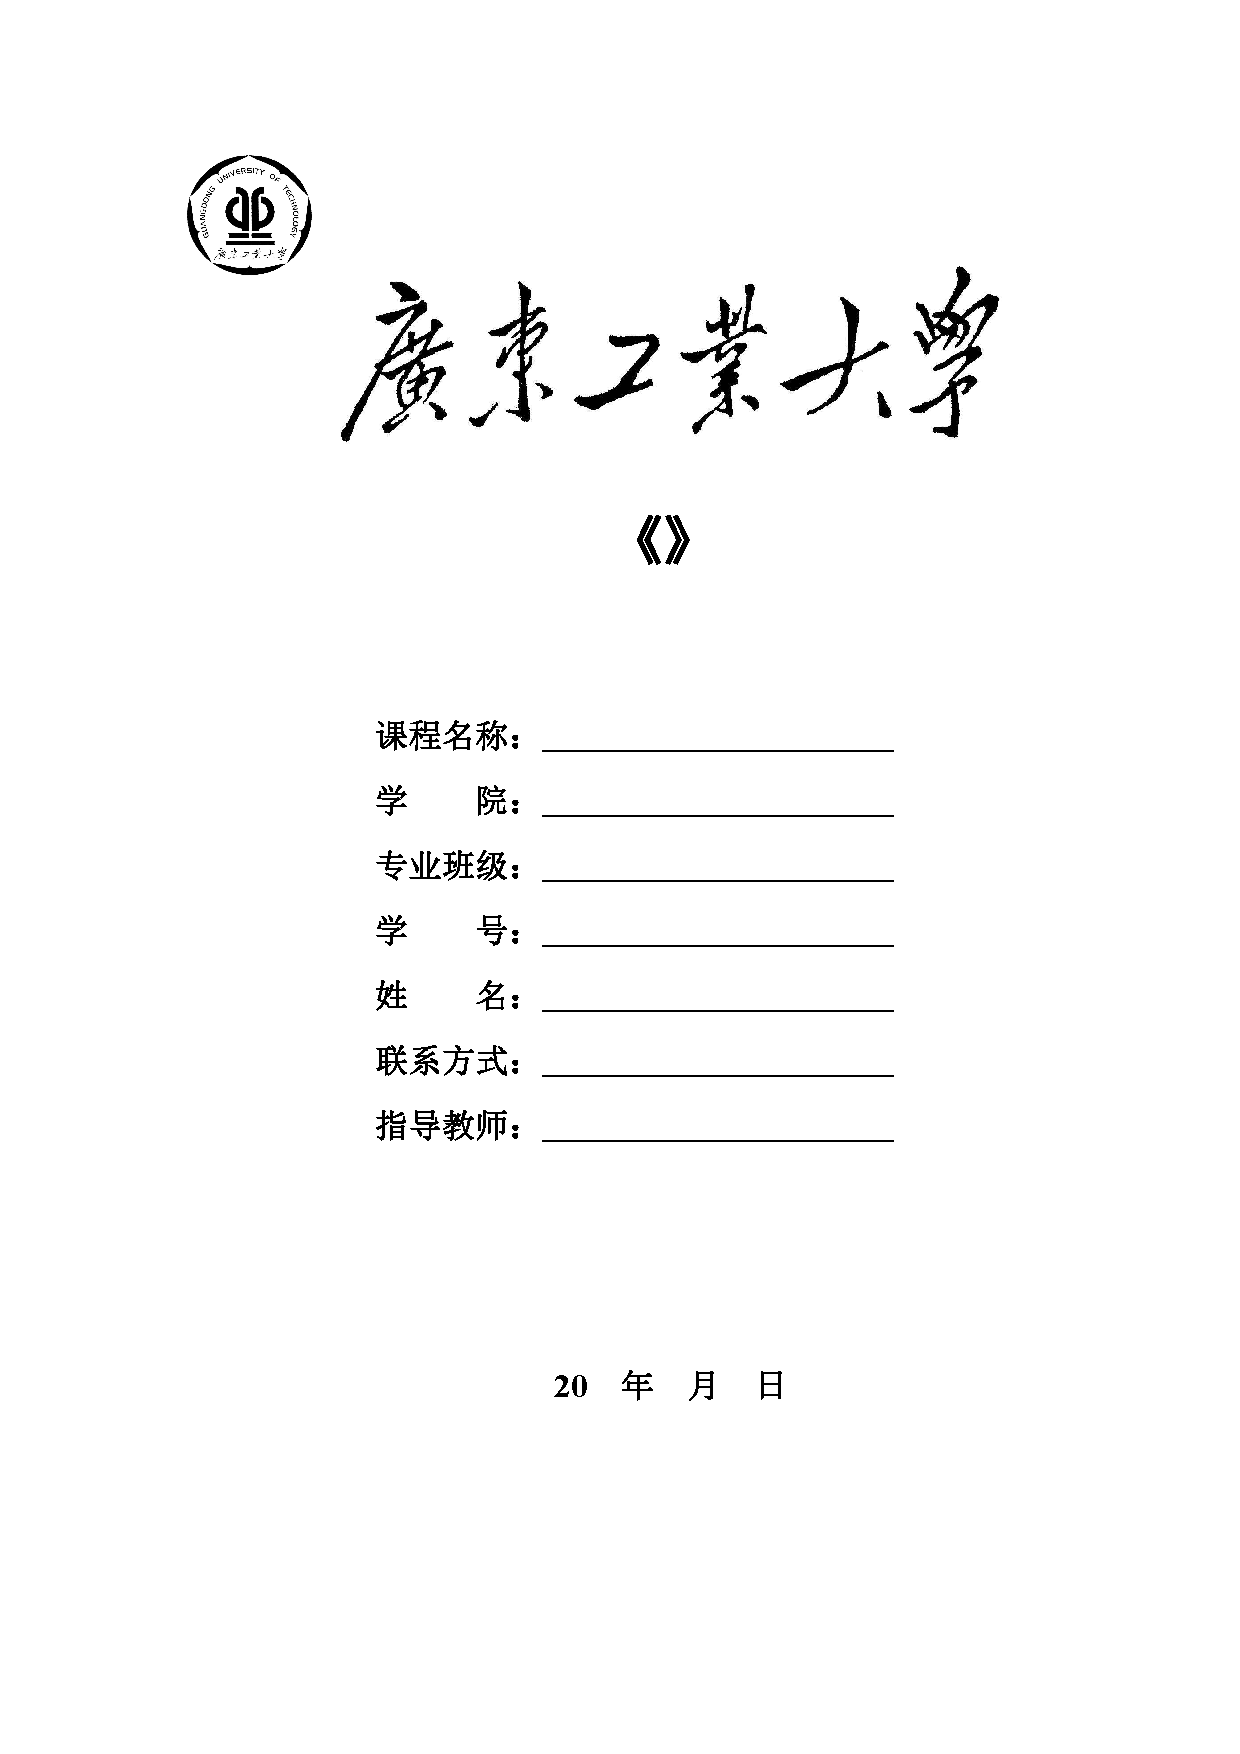
\includepdf[pages=1]{1_1_课程论文封皮.pdf}}{}
\newpage
\pagenumbering{arabic}
{
\Large
\tableofcontents
}
\newpage
\pagenumbering{arabic}
\renewcommand{\abstractname}{引言}
\begin{abstract}
\addcontentsline{toc}{section}{引言}
1\par
\textbf{关键词：}{1\quad 2\quad }
\end{abstract} 

\section{项目背景与功能}%\cite{chinastor} \par
\subsection{项目背景} 
\subsubsection{背景}
1\cite{DBLP:journals/corr/abs-2010-11929}
\begin{itemize}
    \item 1
    \item 2
    \item 3
    \item 4
\end{itemize}\par
\begin{figure}[H]
    \centering
    \begin{subfigure}{0.9\linewidth}
        \centering
        % 若图片不存在则用占位框代替，避免报错
        \IfFileExists{640.jpg}{
\includegraphics[width=0.6\linewidth]{640.jpg}}{\fbox{缺少图片 640.jpg}}
\end{subfigure}
    \caption{\small 罗翔老师}
\end{figure}
\subsubsection{现状}
2
\subsection{功能}
3
\begin{enumerate}
    \item \textbf{1}1
    \item \textbf{2}2
    \begin{enumerate}
        \item \textbf{2.1}1
        \item \textbf{2.2}2
\end{enumerate}

% 结束外层枚举环境（原先遗漏了 \end{enumerate}）
\end{enumerate}

\begin{tabularx}{\textwidth}{lll}
    \toprule
    \textbf{1} & \textbf{2} & \textbf{3} \\
    \midrule
    \textbf{1} 
    & 2 
    & \begin{minipage}[t]{\hsize}
        \begin{itemize}[nosep, leftmargin=*]
            \item \texttt{3.1}: 1
            \item \texttt{3.2}: 2
            \item \texttt{3.3}: 3
        \end{itemize}
      \end{minipage} \\
    \addlinespace
    \textbf{2} 
    & 3
    & \begin{minipage}[t]{\hsize}
         \begin{itemize}[nosep, leftmargin=*]
            \item \texttt{4.1}: 1
            \item \texttt{4.2}: 2
            \item \texttt{4.3}: 3
        \end{itemize}
      \end{minipage} \\
    \bottomrule
\end{tabularx}\par

\begin{figure}[H]
    \centering
    \begin{subfigure}{0.5\linewidth}
        \centering
        \IfFileExists{640.jpg}{
\includegraphics[width=1\linewidth]{640.jpg}}{\fbox{缺少图片 640.jpg}}
        \caption{正面}
    \end{subfigure}
    \hfill
    \begin{subfigure}{0.4\textwidth}
        \centering
        \IfFileExists{640.jpg}{\rotatebox{90}{
\includegraphics[width=1\linewidth]{640.jpg}}}{\fbox{缺少图片 640.jpg}}
        \caption{背面}
    \end{subfigure}
    \caption{\small 2}
\end{figure}


\[ A = k \cdot X + C \]

\begin{equation}
    A = k \cdot X + C
\end{equation}
% 修正 lstlisting 可选参数语法（合并为一个可选参数列表）
\begin{lstlisting}[language=Python, caption={1}]
    # 1
class 1(L2):
    # 新的构造函数
    def __init__(self):
        super(1, self).__init__()
        super().__init__()
\end{lstlisting}

\nocite{*}
\bibliographystyle{plain}
\bibliography{cankaowenxian}



\end{document} 
